\chapter{序論}
\label{chap:introduction}
\section{研究の背景}

\subsection{生成クエリネットワーク}
2018年にAli Eslamiらが提案した生成クエリネットワーク(Generative Query Network)\cite{Eslami2018}は,画像と視点座標という2つのセンサー情報から環境に関する抽象表現(シーン表現)を獲得し,未知の視点座標からの観測画像を予測して生成する深層生成モデルである.このように,異なる視点からの複数の画像から,3次元的な形状を復元して可視化する技術は,コンピュータビジョンの分野ではStructure from Motion(SfM)として知られており,拡張現実(AR)や3Dスキャンなどの技術にも応用されて盛んに研究が行われてきた.しかし,既存のSfMでは3次元形状を点群やメッシュなどを用いて明示的にモデル化してから,それをレンダリングして2次元の画像として表示することが一般的であった.一方で,生成クエリネットワークでは,3次元形状を明示的にモデル化することなく,多層ニューラルネットワークを用いた深層生成モデルによって暗黙的に表現しており,3次元モデルの構築とレンダリングを一気通貫で行う全く新しい手法として大きな注目を集めた.

生成クエリネットワークは,大きく分けて「表現ネットワーク」と「生成ネットワーク」という2つのニューラルネットワークで構成されている.表現ネットワークは,事前に与えられたあるシーンの視点と画像のペア群({\bf コンテキスト}と呼ぶ)を入力として,シーンを表す抽象表現ベクトル({\bf シーン表現}と呼ぶ)を出力する.そして,生成ネットワークは,そのシーン表現と別の視点座標を入力として,対応する未知の観測画像を予測して生成・出力する.これらの2つのニューラルネットワークは,誤差逆伝播法を用いてパラメータの最適化を行うことで,学習される.

このように学習された生成クエリネットワークは,Fig. \ref{fig:gqn_example}のように,少ないコンテキストからでも非常に正確に未知の視点からの画像を生成することができる

\begin{figure}[tbp]
  \begin{center}
    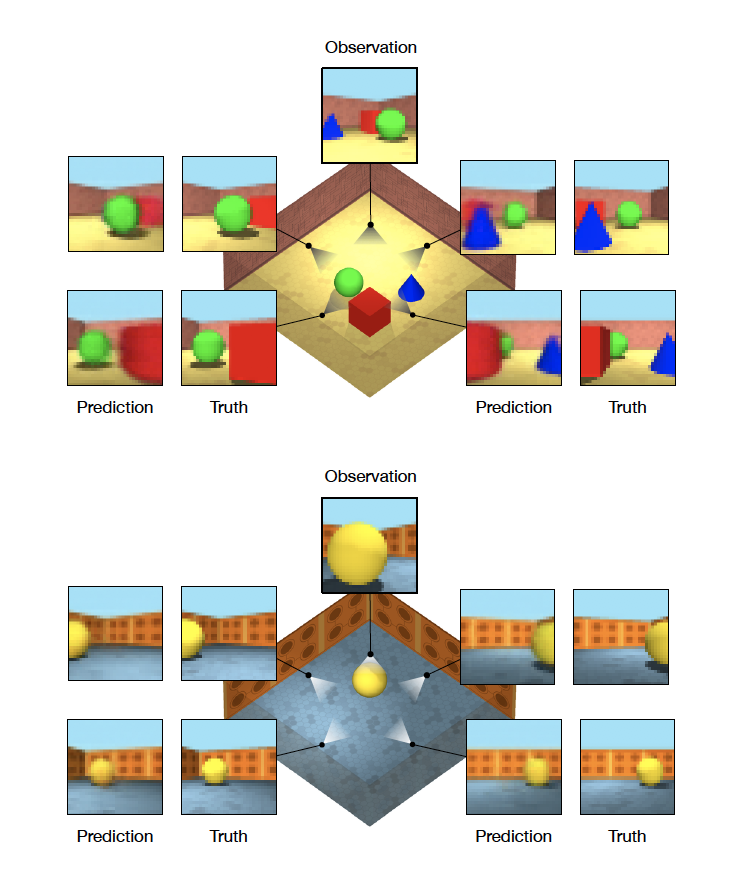
\includegraphics[width=\linewidth]{./figures/gqn_example.png}
    \caption{生成クエリネットワークによる画像生成例}
    \label{fig:gqn_example}
  \end{center}
\end{figure}

\subsection{生成クエリネットワークの問題点}
生成クエリネットワークは,その革新性から様々な実世界応用が期待されている一方で,現状では多くの課題があることが指摘されている.

\subsubsection{学習に要する計算機リソースと時間が膨大}
生成クエリネットワークを提案した論文では,合計96GBのメモリ容量をもつGPUを使用して,3日間モデルの学習を行っており,一般的な計算機リソースでこれを実現することは非常に困難である.一般的に,モデルの学習に使用できるGPUのメモリ容量は$12 \sim 24$GB程度であり,限られた計算機リソースにおいても許容可能な時間内で一定の性能を発揮することを可能にする必要がある.

\subsubsection{学習が不安定である}
生成クエリネットワークの学習においては,ハイパーパラメータが結果に大きく影響を与えることが再現実装を行う中でもわかっている.例を挙げると,Fig. \ref{fig:gqn_failure}のようにモデルの潜在変数の次元数を大きくした場合に学習が全く進まなくなってしまう現象が確認されている.このように,安定した学習を行うことが難しいという点も生成クエリネットワークの課題の1つである.

\begin{figure}[tbp]
  \begin{center}
    \begin{tabular}{cc}
      \begin{minipage}{0.5\linewidth}
        \begin{center}
          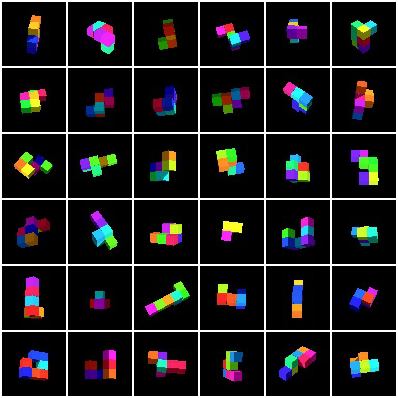
\includegraphics[width=\linewidth]{./figures/gqn_failure_gt.png}
        \end{center}
      \end{minipage}
      &
      \begin{minipage}{0.5\linewidth}
        \begin{center}
          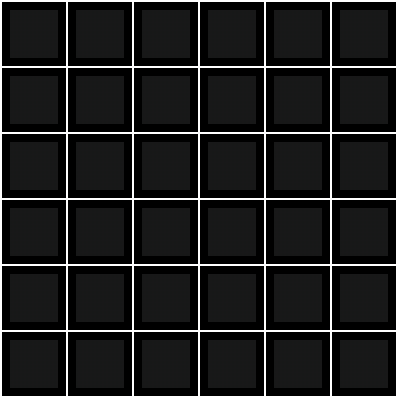
\includegraphics[width=\linewidth]{./figures/gqn_failure.png}
        \end{center}
      \end{minipage}
      \\
      正解画像&予測画像\\
      \end{tabular}
    \caption{生成クエリネットワークの潜在変数の次元数を増やした場合の学習の失敗例}
    \label{fig:gqn_failure}
  \end{center}
\end{figure}

\subsection{研究の目的}
前述した問題点は,深層生成モデルの学習に共通の課題である一方で,生成クエリネットワークではその問題点が特に顕著に現れており,学習に深刻な影響を与えてしまっている.特に,潜在変数の次元数を大きくすると学習が失敗するといったことは,一般的な深層生成モデルの学習においてはあまり起こらない現象であるため,これらの問題点には生成クエリネットワーク特有の原因が存在することが考えられる.そこで,本研究では生成クエリネットワークについて,理論的な検証を行うことで,生成クエリネットワークの問題点の原因を追求し,それを踏まえて問題点を改善する新しいモデルを提案することを目的とする.

生成クエリネットワークの検証においては,特にその前提となっている確率モデルに着目する.これは,深層生成モデルの構築の際には,まず与えられるデータの生成過程を仮定する確率モデルを設計し,それに基づいてモデルのアーキテクチャを構築することが必要であるが,生成クエリネットワークでは,この確率モデルの設計が曖昧に行われており,元論文内でも十分な議論が行われていないためである.そこで,本研究では,生成クエリネットワークが対象とする問題設定が,メタ学習の枠組みと合致していることに注目し,その確率モデルをメタ学習の観点から再構築して検証する.そして,その検証に基づいて,生成クエリネットワークの問題点を整理し,改善手法の提案を行う.さらに,ウェブ上に公開されたデータセットを用いた実験を通して,提案手法の有効性について定性的・定量的な評価を行う.

最後に実験結果を踏まえて,今後の課題と社会応用について述べる.
  
\section{本論文の構成}
本論文の構成は以下のとおりである.

% 第\ref{chap:prerequisite}章では,本研究の前提となる深層生成モデルやメタ学習についての知識を述べる.

% 第\ref{chap:meta_gqn}章では,生成クエリネットワークの確率モデルについてメタ学習のフレームワークを用いて考察を行い,問題点を指摘する.

% %第\ref{chap:related}章では,を行う.
% 第\ref{chap:proposal}章では,前章の議論を踏まえて,生成クエリネットワークを改善する提案手法について説明する.

% 第\ref{chap:experiment}章では,提案手法に対する評価実験の結果を示し,実験結果への考察を行う.

% 第\ref{chap:discussion}章では,本研究の今後の課題と具体的な社会応用可能性について議論する.

% 第\ref{chap:conclusion}章を本論文のまとめとする.